\chapter{Effects of sterols on fengycin aggregation}
\label{c:chapter3}
%\addcontentsline{toc}{chapter}{Cholesterol hinders fengycin aggregation}
\section{Introduction}
World human population has reached 7.71 billion, as of April 2019. In  order to provide food for
this growing population we need better yield in agriculture\cite{Haqq-Misra2019}.Even though agricultural practices have improved, every year 
crops are destroyed by various microbial infections, of which 60\% are caused by fungal species.\cite{Anthony2011} To cope with this, various 
antibiotics have been synthesized like amphotericin B, natamycin and nystatin\cite{Burke2012, 
Hammond1977, Prieto2006}. However these synthetic compounds are more prone to 
antibiotic resistance from different fungal and bacterial species, hence the focus has shifted to 
antimicrobial lipopeptides which have higher selectivity\cite{Avis2007}.

Lipopeptides target the pathogen's cell membrane, causing membrane leakage and ultimately cell death. They are 
better evolved to evade antibiotic resistance since they target fungal/bacterial membranes \cite{Hancock2006}.
Fengycins are a class of lipopeptides that specifically kill certain fungal specie. \cite{Jacques2008, Thonart2005} Fengycins alongwith surfactins and iturins are synthesized by a bacteria \textit{Bacillus subtilis} as an immune response towards fungal attack\cite{Jung1986, RomeroPerez2007}. It is an essential component of Serenade\textsuperscript{\textregistered} (Bayer) a commercial fungicide and bacteriocide.
It is used to treat plant diseases like clubroot disease (\textit{Plasmodiophora monoliforme}), 
barley head blight (\textit{Fusarium graminearum}), cucurbit powdery (\textit{Podosphaera 
fusca}), black Sigatoka (\textit{Mycosphaerella fijiensis}), grey mold (\textit{Botrytis 
cinerea}) and soft rot (\textit{Rhizopus stolonifer})\cite{Long2013, Yang2007, 
Seguin2009,RomeroPerez2007, Thonart2004, Lu2011, Seddon1998, Yu2008, Allan2002, Lu2011, Bie2011}. 
During the application of Serenade\textsuperscript{\textregistered}, farmers and garderners are exposed to these lipopeptides. 
Different insects, birds and animals in the environment are subjected to these lipopeptides too, so understanding
the effects of fengycin on mammalian cells is important in order to fully comprehend its implications to 
the environment.
%%% This paragraph seems incomplete%%%%%%
In addition, fengycins have low hemolytic activity so it proposed to be used as a skin ointment against fungal 
infections\cite{Jung1986, Jacques1999, Dufrene2005}. In fact previous calorimetric study, suggested fengycin's 
interaction with the stratum corneum (outermost skin layer) mimicking model depends on the lipid phase behavior of 
the lipid vesicles\cite{Eeman2014}.
The main difference between mammalian cells and fungal cells is the presence and absence of cholesterol. In fact 
cholesterol plays a central role in formation of different lipid phases in the membrane \cite{Barenholz2002}.
Eeman et al found that in monolayers mimicking the outermost layer of skin(Stratum corneum), 
fengycins partition into the cholesterol rich fluid phase. \cite{EemanDeleu2009} This suggests that either fengycin 
prefers a more lipid disordered phase or preferentially interacts with cholesterol.
These suggests that further studies need to be conducted to get a clearer picture of fengycin's mechanism
of action and to determine whether fengycin can be a potential drug target.

Previous studies includes Heerklotz et al's fluorescence lifetime experiments with model membranes of varying phospholipids 
and sterols composition. \cite{Heerklotz2008, Heerklotz2001} The fluorescence dye is usually entrapped inside the 
membrane vesicles and a titration against fengycin determines its dye-releasing efficacy and membrane leakage propensities. 
There are two mechanisms by which lipopeptides after binding disrupt the membrane: a) graded leakage -- caused by 
thinning of membrane and disordering of lipid such as caused by surfactin\cite{Heerklotz2011,Seelig2007} b) 
All-or-non mechanism are caused by long-lived large pores, without a pore no leakage\cite{Heerklotz2011}. Patel et 
al \cite{Heerklotz2011} showed that fengycin follows a all-or-none mechanism but they were unable to confirm 
whether pores were formed due to aggregates of fengycins on the membrane surface.
 Fiedler et al found that the tolerable fraction of fengycins on the membrane surface increases 
in a mixture of POPC and cholesterol model membranes compared to pure POPC.\cite{Heerklotz2015}
Similarly Mantil et al found that both for model membranes and supported lipid bilayers extracted from microbial 
lipids, presence of ergosterol buffers the membrane disordering ability of 
fengycins.\cite{MantilTyler2019,MantilAvis2019}
But both the papers couldn't determine the exact mechanism of how fengycin  is retained 
to a higher threshold level in the cholesterol rich membrane without disrupting it.
One of the suggestions by Fiedler et al was that fengycins cannot aggregate in the 
cholesterol rich surface which results in its slow effux of the dye in vesicles when fengycins are 
added\cite{Heerklotz2015}.

Understanding the specific fengycin-lipid interactions after binding can be an interesting problem to study using molecular dynamics simulations. 
These simulations can be thought of more like a high resolution microscope in which we can control our system to the highest degree. 
Strides have been made in molecular dynamics to study different antimicrobial
peptides and their interactions with membrane \cite{Schulten1993, Tieleman2007, Pastor2016}.
And yet one of the issues of simulating these lipopeptides is sufficient sampling so that we can observe lateral displacement of lipids and mixing of the lipids in the bilayer. The other issue is peptide's conformational sampling within the bilayer. Due to it's cyclic structure, fengycin occupies a much smaller conformational space compared to an unstructured peptide which ensures faster convergence. In order to sample lipid displacements we would require several microseconds of simulations.
Coarse-grained simulations help us smoothen the energy landscape leading to a much faster sampling of the conformational space \cite{Marrink2013}.
In addition, we also used weighted ensemble method to get a better sampling of the free energy surface in order to correlate protein-protein lateral motion and lipid-lipid mixing\cite{Chong2017}.
 
 Using molecular dynamics simulations Horn et al \cite{Grossfield2013} and 
 Sur et al \cite{Grossfield2018} concluded 
 that bigger aggregates are more likely found in model fungal membranes which  
 ultimately leads to membrane. Hence, in this study we looked at the interactions 
 between fengycins and between fengycin and cholesterol/phospholipids on the membrane 
 surface. Specifically, we were interested whether in correlating aggregation 
 propensity to cholesterol's presence/absence in the membrane and its insinuation to
 the membrane's various properties.
 
 \section{Materials and Methods}
\label{s:methods}

\subsection{System construction}
\label{ss:sys_cons}
All the particles in our systems were modeled using MARTINI 
coarse-grained force-field Ver. 2.2P.Model fungal membranes,
palmitoyl-oleoyl-phosphati- dylcholine (POPC) and model mammalian membranes, POPC:Cholesterol(CHOL) are used.
 More details about the system composition
can be found in Table \ref{t:sys_cons}.

The parameters for Fengycin has been adapted from Horn et al parameter files \cite{Grossfield2013}.
For lipid parameter files we used the MARTINI Ver. 2.0 and for the peptide part of fengycin  MARTINI Ver. 2.2 was used.
The chemical structure of Fengycin A that we used is shown in Figure \ref{f:chem_str}.
Fengycin A was modeled according to Josh et al's coarse-grained model \cite{Grossfield2013}
with glutamate 8 being replaced by glutamine which resulted in a net charge of -1 for Fengycin A.


\begin{figure}[h!]
\centering
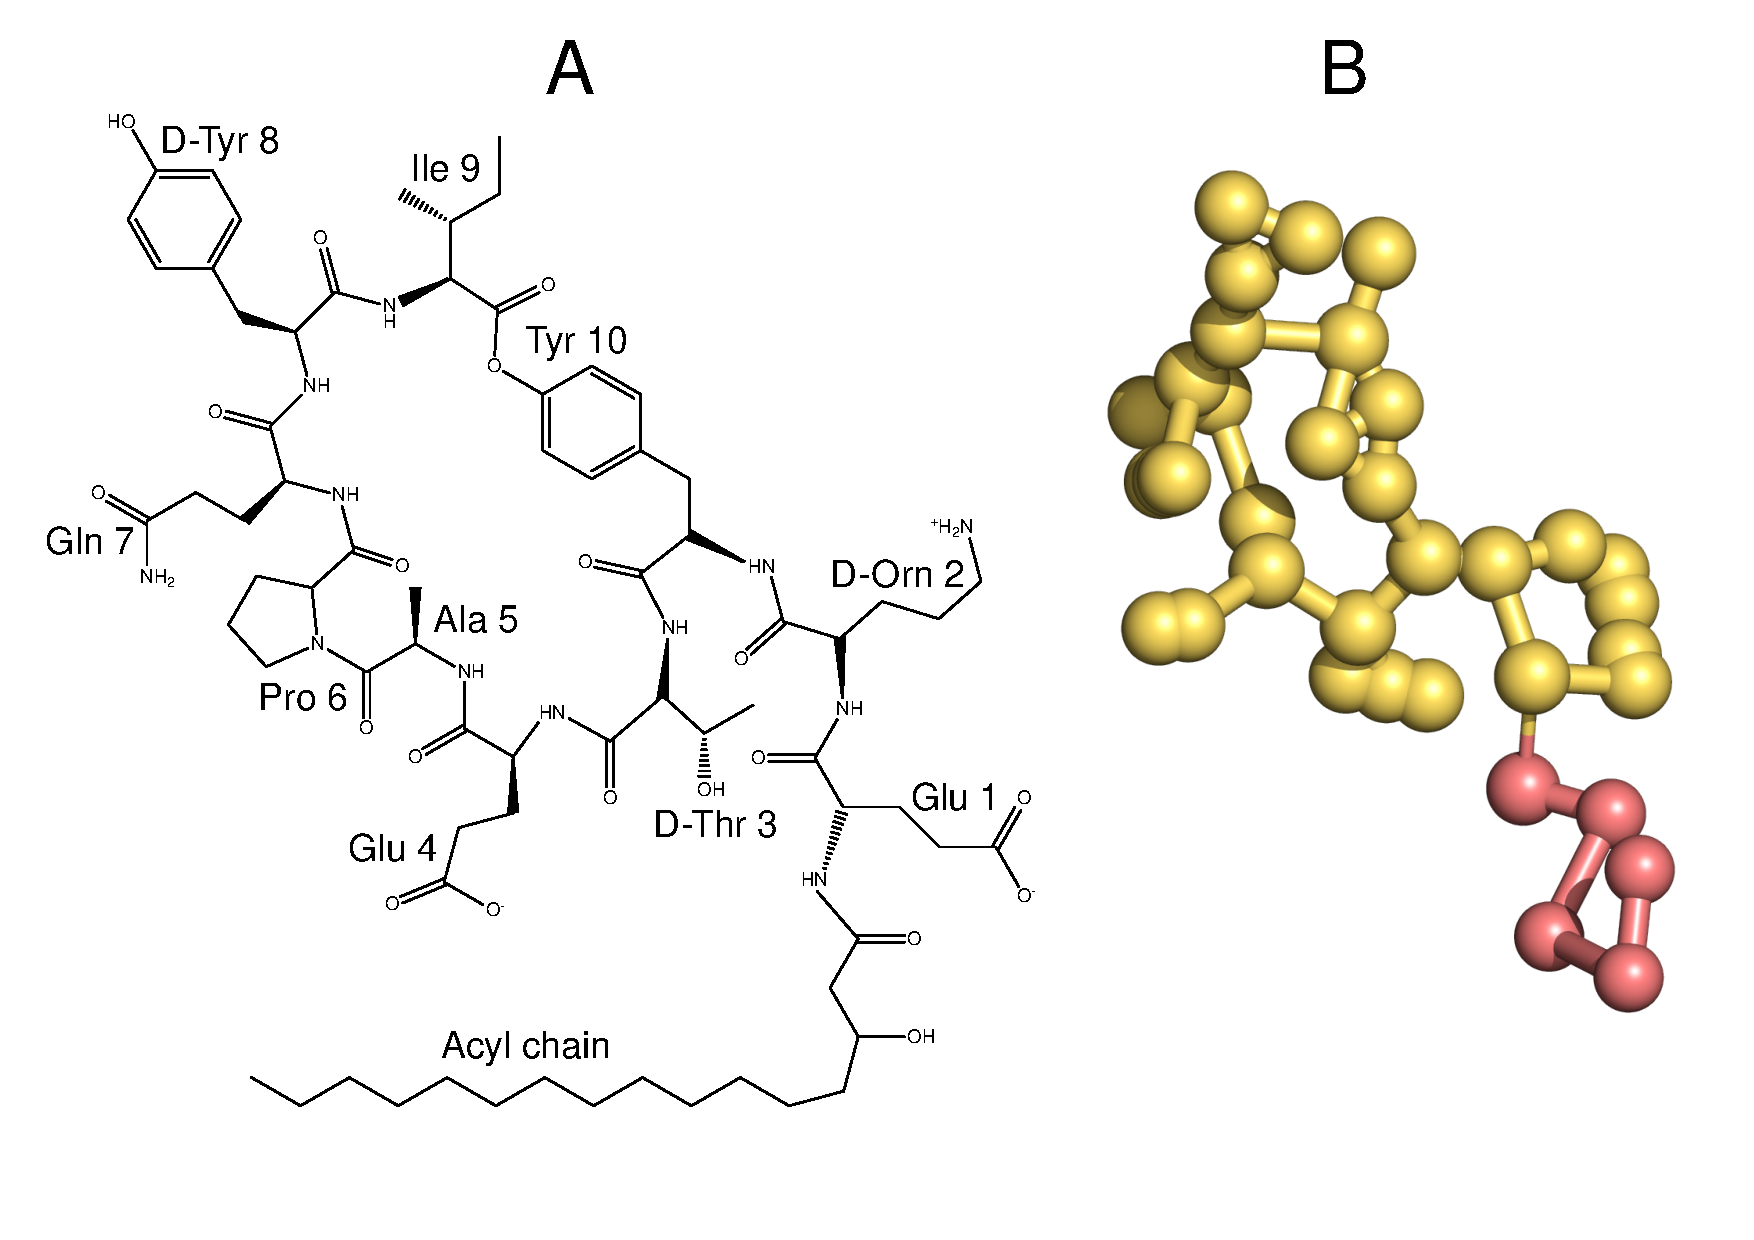
\includegraphics[width=1.0\textwidth]{chapter3_figs/comb_str_feng.pdf}
\caption{Chemical structure of fengycin A}
\label{f:chem_str}
\end{figure}

Initially, we randomly place fengycins on an xy-plane. Then we use insane tool to build a grid of phosholipids, cholesterol(if present), polarizable water and 150 mM NaCl salt around the fengycins\cite{Marrink2015}.
We let the system equilibrate with an initial 10000 minimization procedure using GROMACS Ver. 2016.3 \cite{Lindahl2015}.
Next we ran molecular dynamics simulations of length 10-15 ns with 2 fs as time steps.
Then increased the time step to 20 fs while running production.

%%%%Update this table after taking into account all the data.
\begin{table}[h!]
  \caption{Summary of simulations}
  \label{t:sys_cons}
  \begin{tabular}{llccc}
    \hline
    \textbf{System}  & \textbf{Phospholipids} & \textbf{fengycins per leaflet} & \textbf{Length($\mu$s)} & \textbf{\# of replicates} \\
    Mammalian   & PC:CHOL & 15 & $\sim$ 330  & 3 \\
    Fungal & PC  & 15 & $\sim$350 & 3\\
    Neat  & PC & 0 & $\sim$0.6 & 3\\
    Neat & PC:CHOL & 0 & $\sim$0.6 &3\\
    \hline
  \end{tabular}
\end{table}

\subsection{Weighted ensemble method}
\label{ss:we_method}
We used the Weighted ensemble path sampling technique to calculate the probability distribution for fengycin aggregates. This method is implemented in WESTPA software package \cite{WESTPA2015,WESTPA_github}.
In this method no additional bias or force is added to the system. An appropriate reaction coordinate is chosen
depending on the process we are observing. For our case we were looking at the aggregation behavior of fengycins
on the membrane surface, hence we chose number of contacts as the reaction coordinate which can capture quantitatively
the aggregation process. Each centroid-centroid contacts between i and j fengycins is defined as

\begin{equation}
\label{e:contact}
S_{ij} = \frac{1}{1+ \left ( \frac{r_{ij}}{r_0} \right)^6}
\end{equation}
where $r_{ij}$ is the distance between the centroid of the peptide part of fengycins and $r_0$ is the distance at which there is half contact between the atoms. In our case which chose it to be 10 \AA
The total number of contacts for a given frame in the trajectory is the sum of all possible contacts between all the fengycins.
\begin{equation}
\label{e:no_cont}
C_{AB} = \sum_{i \in A} \sum_{j \in B} S_{ij}
\end{equation}
In order to promote transition from low energy state to high energy state we divided the reaction coordinate space into bins.
Next, we used different coordinate files (.gro) occupying different bins as our starting points to run short 5ns long simulations. 
Then we re-evaluate the MD trajectories to see if the value of the progress coordinate has changed or not in each of the trajectories.
From there on, if the system has a different progress coordinate and it falls into an unoccupied bin then the system is replicated M times where M is the maximum number of trajectories in a bin. Hence, weight of each trajectory in that particular bin is reassigned as 1/M taking into account the original weight of the incoming walker.
 If the walker goes to an occupied bin
 and the number of walkers in that bin is already M then the weight of the incoming walker is assigned to any of the already
 existing walker in the bin and that walker is terminated.
 This whole method increases the probability of a walker going from one state to another
 by replicating or pruning trajectories depending on the time they spent in each bin \cite{WESTPA2015, Chong2017}.

 \subsection{Simulation details}
 \label{ss:ssim_details}
We used the Gromacs Ver. 2016.3 to run each of the short 
trajectories\cite{Lindahl2015}. Since MARTINI models are based on 
coarse-grained particles which lack some of the degrees of freedom found
in all-atom simulations, the systems exist in a much smoother landscape and 
the goal is to get as much sampling done as possible but compromising on 
some of the details in the energy landscape\cite{Marrink2013}. Thus a longer timestep
is more effective in sampling the energy landscapee and we used a 20fs 
time step.\cite{Wilfred2009} The neighbor list was updated 
every 20 steps. The simulations were run in an isobaric-isothermic 
ensemble with Parrinello-Rahman barostat \cite{Rahman1981,RahmanParrinello2007} and Velocity 
rescaling thermostat \cite{Parrinello2007}. Electrostatics interactions 
were calculated using Reaction field method as implemented in Gromacs, 
ver 2016.3.\cite{Watts1973} The Verlet scheme was used to compute the Van
der waals forces using a 11 \AA cutoff. The cumulative time of the 
simulation is shown in Table \ref{t:sys_cons}. This is the sum of the number of 
trajectories in all bins in each iteration multiplied by the length of 
each trajectory and the number of total iterations completed for the three 
replicates in each membrane systems.

\subsection{Simulation analysis}
\label{ss:sim_analysis}
Lightweight Object Oriented Structure Library (LOOS) was used to analyze all the data along with the analysis tools that came with the WESTPA software \cite{WESTPA2015,Grossfield2014, Grossfield2009, LOOS_github}. All the analysis were performed at 1 ns resolution. For the average quantities we used the last 50 WE iterations. The averages are computed by taking into account the weight associated with each trajectory. Unless otherwise specified error bars are associated with standard error calculated by treating each weighted ensemble simulation as one independent measurement.

\subsubsection{Molecular order parameters}
\label{sss:mol_ord}
This is calculated by first estimating the average angle between the
second and third principal axes of the phospholipid POPC w.r.t the 
membrane normal. The reason being that this most aptly corresponds to 
the C-H angle for deuterium exchange exeriments in solid state NMR. 
Then the following equation is used to compute the Molecular order 
parameters ($S_{mol}$) \cite{Seelig1977}.

\begin{equation}
\label{e:s_mol}
    S_{mol} = \left | \left \langle \frac{3 \cos^2 \theta -1}{2} \right \rangle \right |
\end{equation}
We used the tool ${dibmops}$ in LOOS to create the histogram of molecular order parameter of phospholipids w.r.t the distance from fengycins.

\subsubsection{Radial Distribution function}
\label{sss:rdf}
We used the tool ${xy\_rdf}$ to calculate the lateral radial distribution function for POPCs, cholesterols and fengycin of various combinations. This tool takes into account the centroids of these species and not individual atoms.

\subsubsection{Probabiliity distribution for fengycin-fengycin contacts and fengycin-lipid contacts}
\label{sss:prog_coord}
We used the tool ${w\_pdist}$ in the WESTPA software that creates 
iteration wise weighted histograms of the progress coordinates taking 
into account all the trajectories. Then we used the tool 
\textit{plothist} also part of WESTPA software that plots an average 
probability of progress coordinates  for a particular range of 
iterations. We also used \textit{plothist} to create a heatmap of 
iterations vs average probability distribution vs progress coordinates.

\subsubsection{Fengycin-lipid contacts}
\label{sss:fl}
We also calculated the contacts between lipopeptides and phospholipids using the equations 
\ref{e:contact} \& \ref{e:no_cont} for all trajectories and all 
iterations with selections corresponding to fengycins phospholipids. We took into account cholesterol if present. Then using WESTPA tools  ${w\_pdist}$ and $plothist$ we 
also created a weighted histogram of probability of fengycin-fengycin and 
fengycin-lipids contacts.

\subsubsection{Aggregation propensity}
\label{sss:na}
We considered two fengycins in contact if they have 50 atoms in contact 
which are 6.5 \AA apart using the script $no_of_mers_class.py$. Then we counted how many fengycins are in 
contact with each other. If there were fengycins which were in 
contact with multiple fengycins we considered them as aggregates. Then 
again using WESTPA tools  ${w\_pdist}$ and $plothist$ we 
created a weighted histogram of fengycin-fengycin contacts and 
no. of aggregates \cite{WESTPA2015,WESTPA_github}.

\subsubsection{Z-distance of phosphate heads}
\label{sss:z-dist}
We calculated the height of the phosphate bead of POPC with respect to center of membrane for all phospholipids in all replicates of systems with or without cholesterol. We then histogrammed these heights with respect to the lateral distance between fengycin's centroid and individual phospholipid centroid. In addition the weights of each trajectory from which the heights of phospholipids were extracted was also considered in order to get the average histogram. 
All the analysis scripts are available as a github repository at 
%%%%{link for github repo}

\section{Results}
\label{s:results}
\subsection{Aggregation is highly ordered}
\label{ss:agg_ordered}

%%%%% Main idea is to question the structures observed%%%%%
Our last paper by Sur et al discussed that larger aggregate has a 
longer lifetime in POPC bilayers compared to the 
same-sized aggregate in POPE:POPG \cite{Grossfield2018}. Similarly, 
Fiedler et al also suggested that in presence 
of cholesterol lower membrane leakage can be attributed to less aggregation 
of the lipopeptides \cite{Heerklotz2015}.
Hence, figure  \ref{fig:xyrdf_ff} shows the radial distribution function between the 
lipopeptides using the method \ref{sss:rdf}. 
The high radial distribution function value suggests strong aggregation 
tendencies between fengycins. Additionally equidistant peaks indicate higher ordered 
linear structures for larger aggregates like trimer, quantamer or pentamers. 
Sur et al similarly conditioned simulations but with all-atom model and they didn't 
observe such ordered aggregates. \cite{Grossfield2018}
Yet simulations performed earlier than that by Horn et al noticed similarly stuctured 
aggregates when they simulated 
a coarse-grained model of a different fengycin type.
\begin{figure}[h!]
\centering
\begin{subfigure}{.5\textwidth}
  \centering
  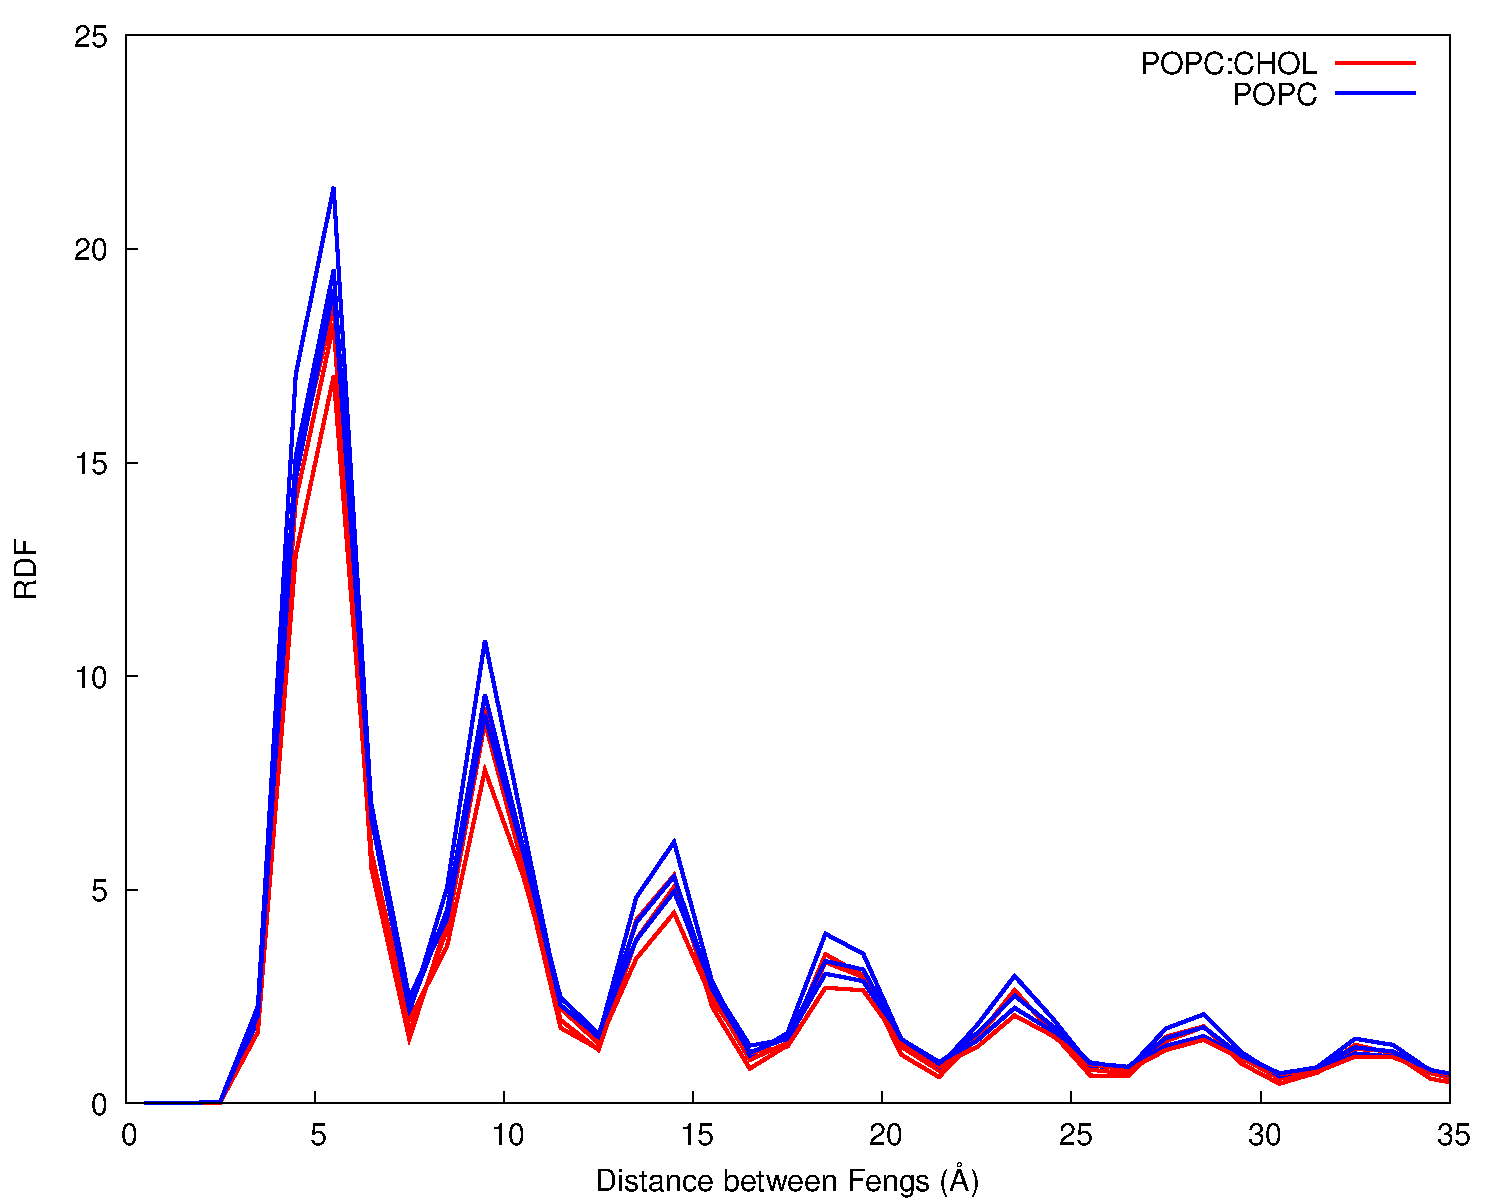
\includegraphics[width=1.0\textwidth]{chapter3_figs/xyrdf_all_ff.pdf}
  \caption{A}
  \label{fig:xyrdf_ff}
\end{subfigure}%
\begin{subfigure}{.5\textwidth}
  \centering
  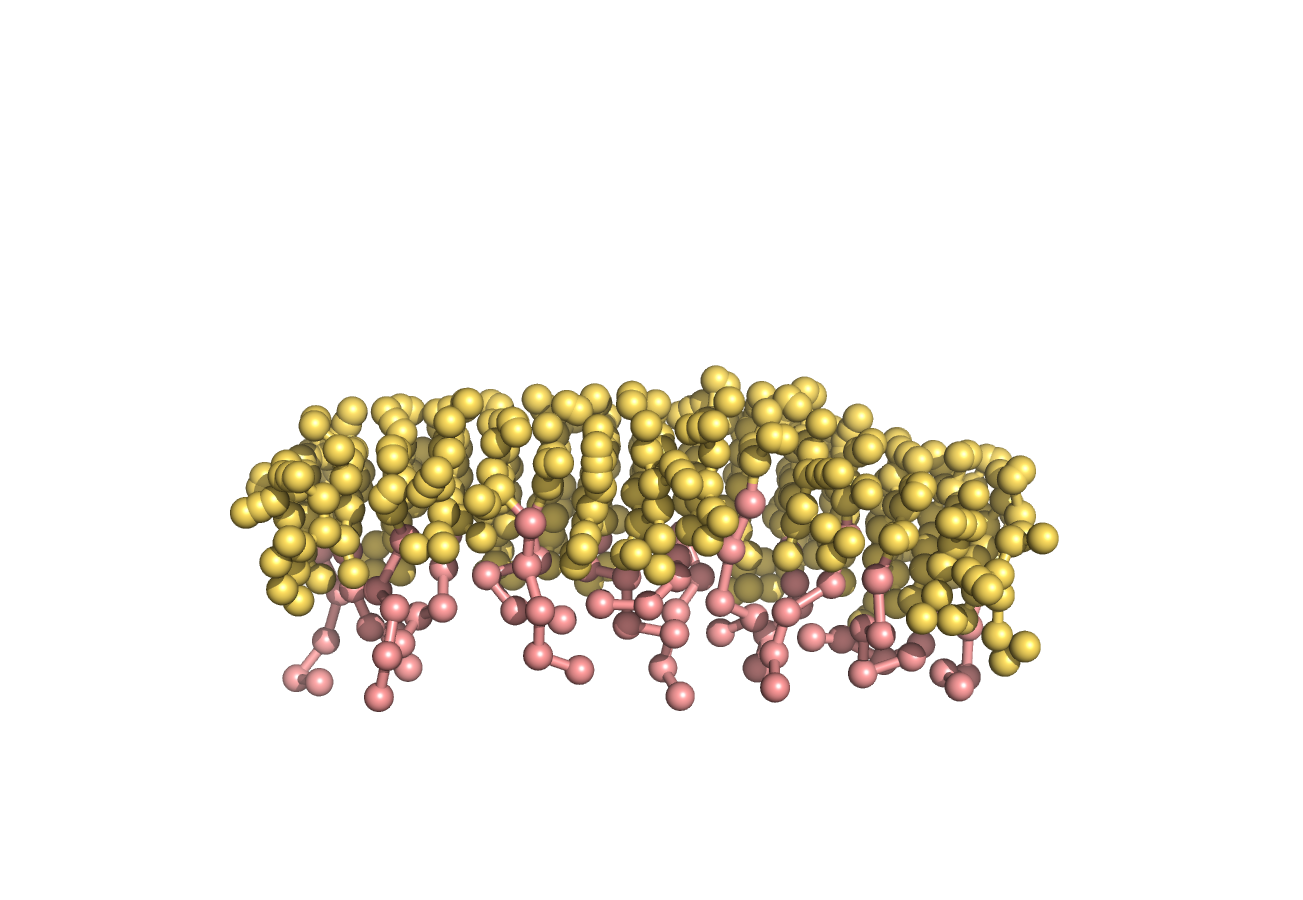
\includegraphics[width=1.0\textwidth]{chapter3_figs/agg_single.png}
  \caption{B}
  \label{fig:agg}
\end{subfigure}
\caption{A. Lateral radial distribution function between fengycins. B. Structure of a single 15-mer aggregate  Along y-axis is the radial distribution function and along the x-axis is the distance between fengycins.  The aggregation propensity of proteins is high in MARTINI model and these ordered structures are not found in our all-atom simulations\cite{Grossfield2018}. Each curve shows the weighted average in each replicate.}
\label{f:xyrdf_ff}
\end{figure}


This suggested that MARTINI force field results in these highly 
structured aggregates almost crystal like, neither observed in the 
all-atom simulation \cite{Grossfield2018} nor in atomic force 
microscopy experiments conducted by Eeman et al where they suggested more random 
orientations and less organized structures for 
fengycin \cite{Dufrene2005}. %%%{Find more structure papers.}

In fact, Javanainen et al reported MARTINI proteins overestimate
protein-protein interactions \cite{Vattulainen2017}.
To fix this issue they tried reducing the protein-protein interactions in the MARTINI forcefield without affecting the other MARTINI parameters. But still the dimer structures found in simulations did not match with the ones obtained via NMR spectroscopy suggesting further improvements in individual amino acid parameters necessary to correctly estimate aggregation free energy \cite{Vattulainen2017}.

\subsection{Aggregation propensity higher in cholesterol}
\label{ss:agg_propensity}
%%%%%%Main idea is to show that aggregation tendencies not that different%%%%%

Fiedler et al also suggested from their fluorescence lifetime experiments that
 slow dye leakage by fengycins on cholesterol rich membranes is due to  more 
aggregation propensity in one over the other \cite{Heerklotz2015}. To bolster this hypothesis, we 
calculated the probability distribution of fengycin-fengycin contacts using the 
method \ref{sss:prog_coord} and Figure \ref{f:cont_prob} shows the result.
\begin{figure}[h!]
\centering
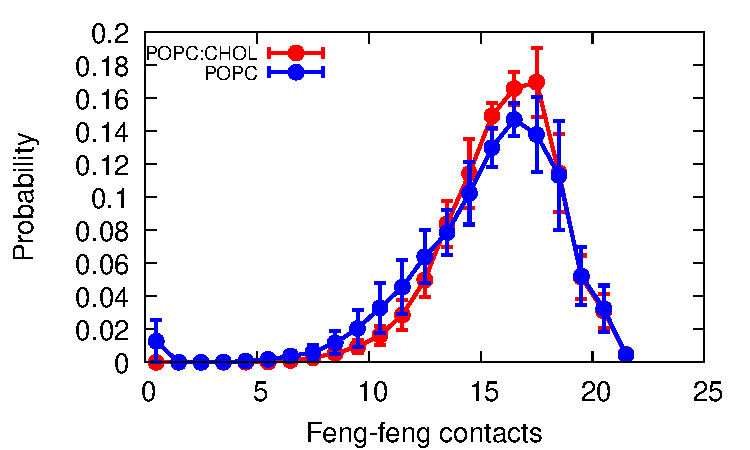
\includegraphics[width=0.6\textwidth]{chapter3_figs/popcchol_pdist_prob.pdf}
\caption{Probability of fengycin-fengycin contacts. Along the x-axis is the number of contacts between fengycins and along y-axis is the weighted average probability of that number of contacts over all trajectories. Number of fengycin contacts is calculated using equations \ref{e:no_cont} and \ref{e:contact}. Error bars is calculated by considering each weighted ensemble run as a single independent measurement.}
\label{f:cont_prob}
\end{figure}
%%%%do t-test on this figure
However figure \ref{f:cont_prob} suggests contrary to Fiedler et al's claims. 
In presence of cholesterol, fengycin has a higher tendency to aggregate on 
the membrane surface. 
Due to shorter distance between adjacent fengycin peptide heads which is indicated in the highly ordered ring stacking that we see in Figure \ref{fig:xyrdf_ff}B we can have high contacts.
%%%%% Sort of correlating the higher aggregation and packing%%%%%
And due to cholesterol's tendency to order the lipids, it can also force the lipid-like tails of fengycins to be parallel to membrane normal . This can result in fengycins spending more time as larger aggregates  than to disintegrate into smaller sized aggregates.

While \ref{fig:xyrdf_ff} shows statistically significant differences between fengycin 
aggregation in the two membrane systems we wanted to quantify this effect in a more 
tangible way. Hence we asked the question \-- can we translate fig. \ref{f:xyrdf_ff} 
into a more comprehensible data? 
To answer this, we looked at the heatmap that showed a correlation between 
fengycin-fengycin contacts and the number of aggregates. 
Fig. \ref{f:na_ff} tells us how many aggregates are formed from 15 
fengycins and what are their sizes. We see that fewer no. of aggregates 
are prefered in the presence of cholesterol with higher fengycin-fengycin contacts implying fewer aggregates with equal or of comparable sizes are more preferred as seen in \ref{f:na_ff}C. 
%%%%% Main idea size of aggregates%%%%%%%
On the other hand in pure POPC for instance 2 aggregates can be very different in composition since the number of contacts range from 15-21 \-- one big and 
 the other smaller or equisized. Figure \ref{f:na_ff} shows 4 aggregates but two of them are monomers so the corresponding number of contacts is pretty low. The difference heat map in Fig. 
 \ref{f:na_ff} suggests that in cholesterol few larger aggregates are more probable. On the other hand
 in pure POPC various aggregate composition are observed.  Hence, we can say that cholesterol subtly changes the way fengycin 
 aggregates prefering more compact aggregates and smaller aggregates are not 
 preferred. This refutes Fiedler et al's claim that 
 aggregation is more preferred in the absence of cholesterol and thus the difference 
 in their membrane leakage phenomenon\cite{Heerklotz2015}.

 
\begin{figure}[h!]
    \centering
    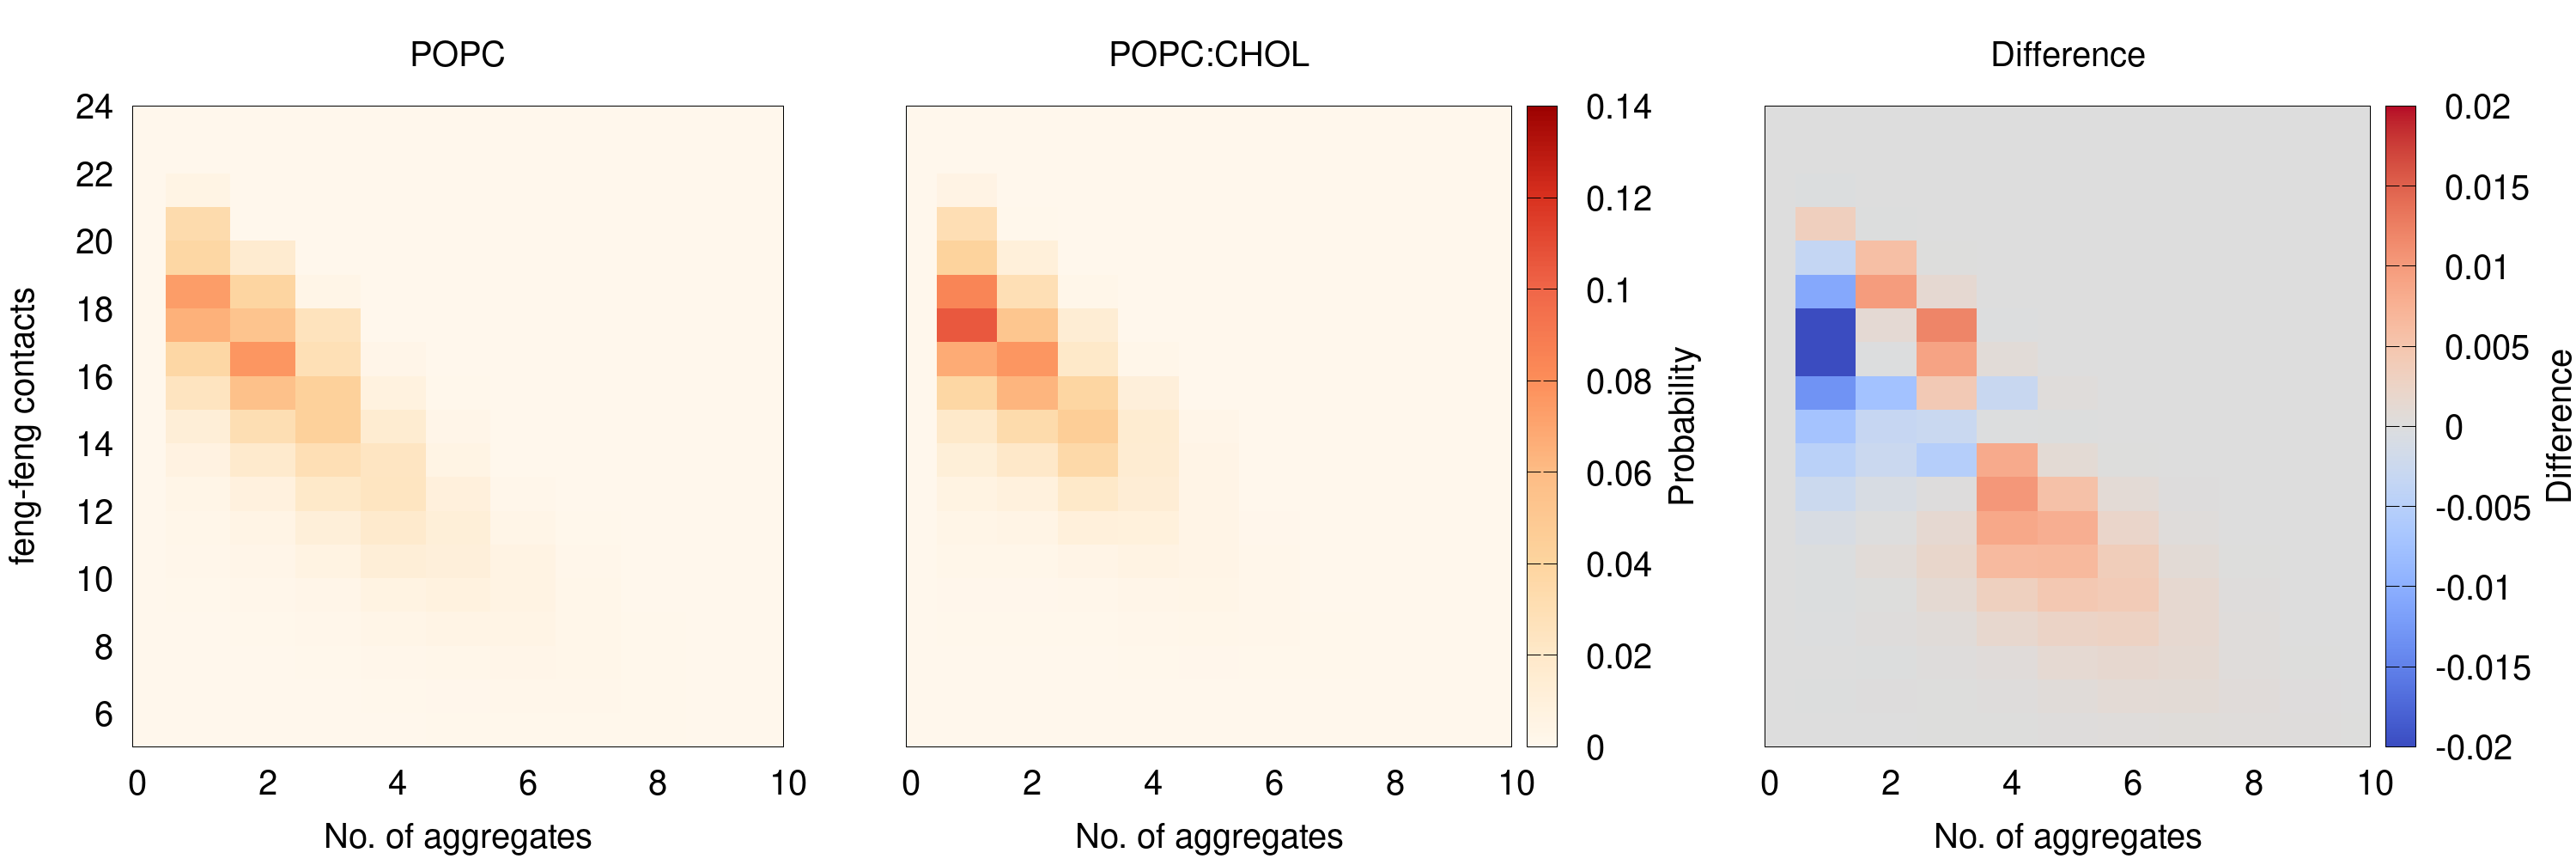
\includegraphics[height=2.0in,angle=0,keepaspectratio]{chapter3_figs/na_ff_prob.png}
    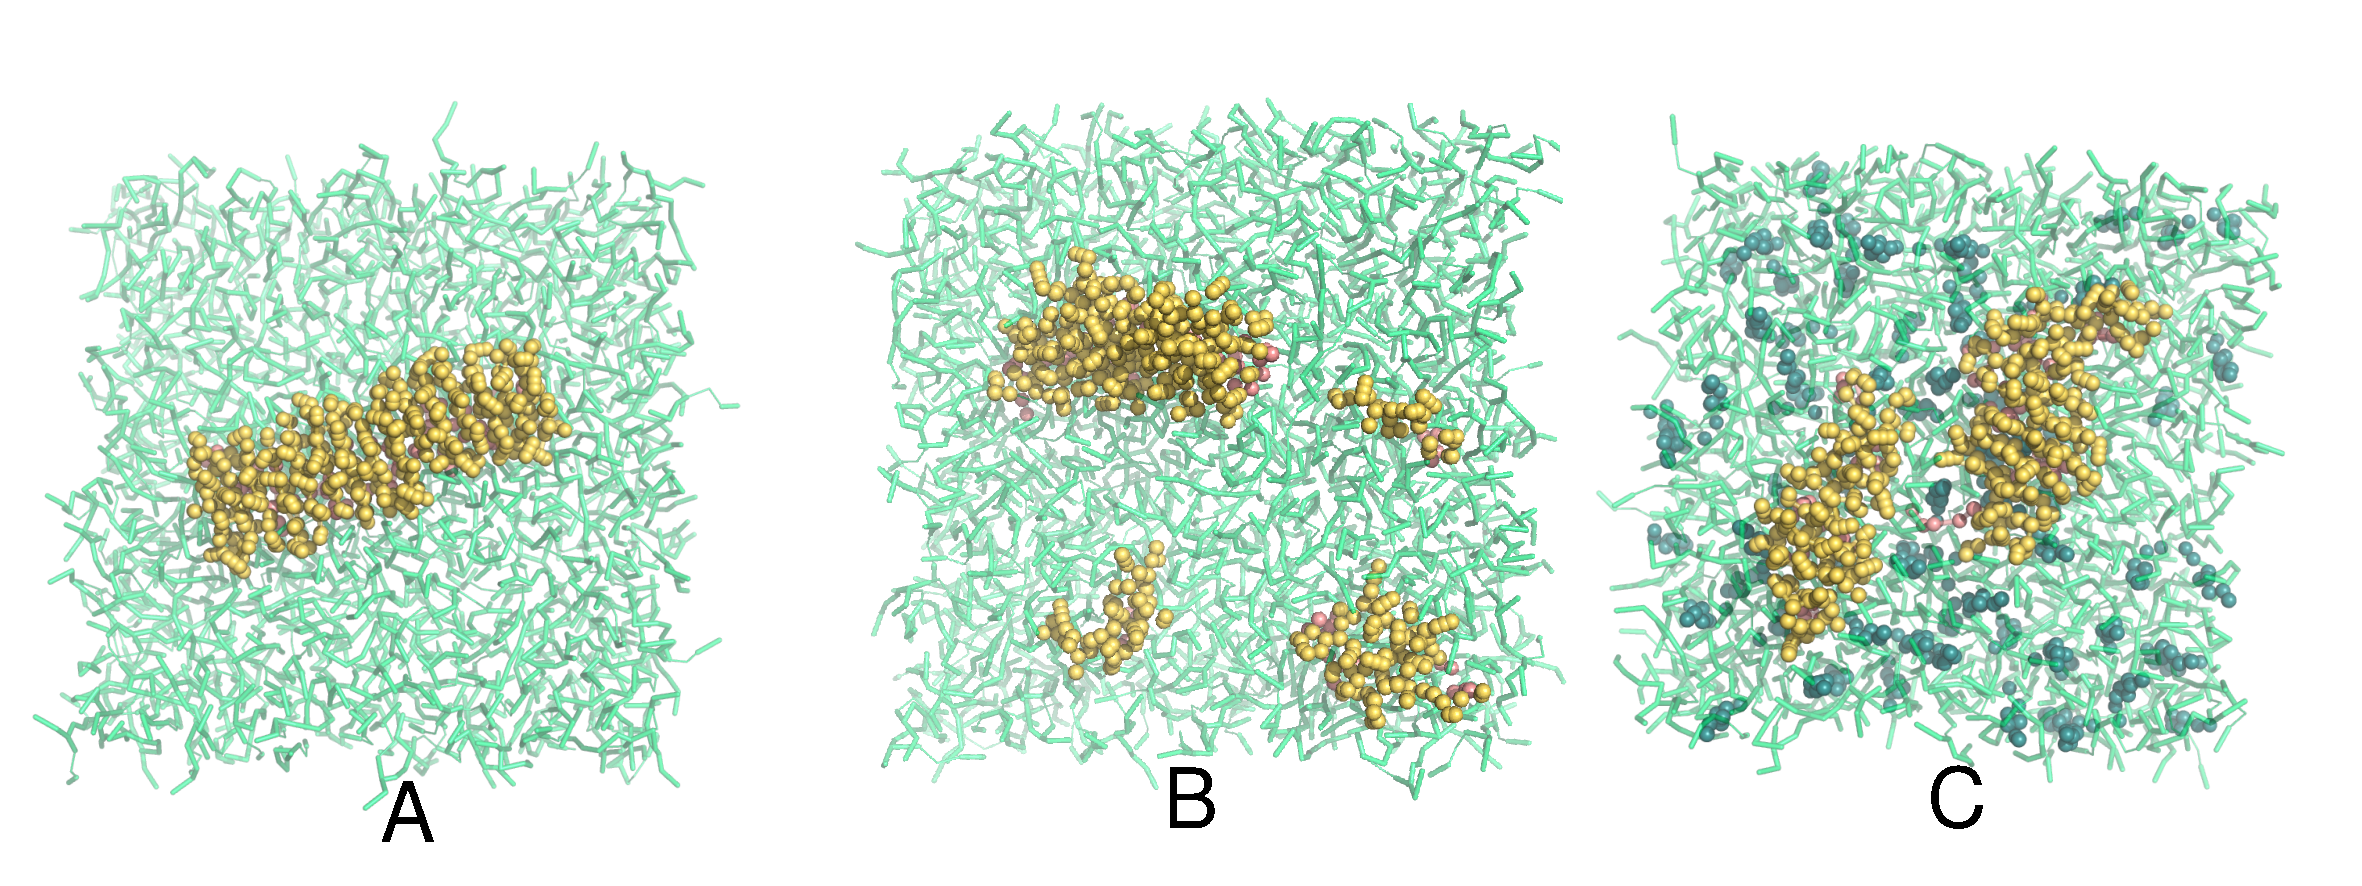
\includegraphics[height=2.25in,angle=0,keepaspectratio]{chapter3_figs/aggs_fig.pdf}
\caption{Probability of number of feng-feng contacts and number of aggregates. Difference is POPC-POPC:CHOL. A, B,C are the different snapshots at the specific aggregation states as stated by the arrows.}
\label{f:na_ff}
\end{figure}

\subsection{Fengycin does not prefer cholesterol or phospholipids}
\label{ss:no_fc_fp}
If the tendency to aggregate is preferred in fengycins, Sur et al suggested that the 
fengycins might have lesser tendencies to specifically interact with other phospholipids. 

Our next question does fengycins preferentially interact with either phospholipids or cholesterol? 
%%%%Important no specific interactions%%%%%%
In order to answer that we plotted the lateral radial distribution function between fengycins and cholesterol or phospholipids' using method \ref{f:xyrdf_fc_fp}. This suggested that phospholipids and cholesterols are both randomly placed around fengycins and presence of fengycins doesn't cause demixing because the radial distribution curves are unchanged with the presence/absence of it. This again refutes the claims of Fiedler et al that there can be specific hydrogen bonds between cholesterol and fengycins which result in lower inhibition of fengycins in cholesterol.\cite{Heerklotz2015} 
Conversely these results are similar to what Sur et al observed for all-atom simulations of a different fengycin in POPC system in which they observed no specific interactions between POPC and fengycin and the higher the aggregation tendencies lower are specific interactions between fengycins and lipids \cite{Grossfield2018}.
\begin{figure}[h!]
\centering
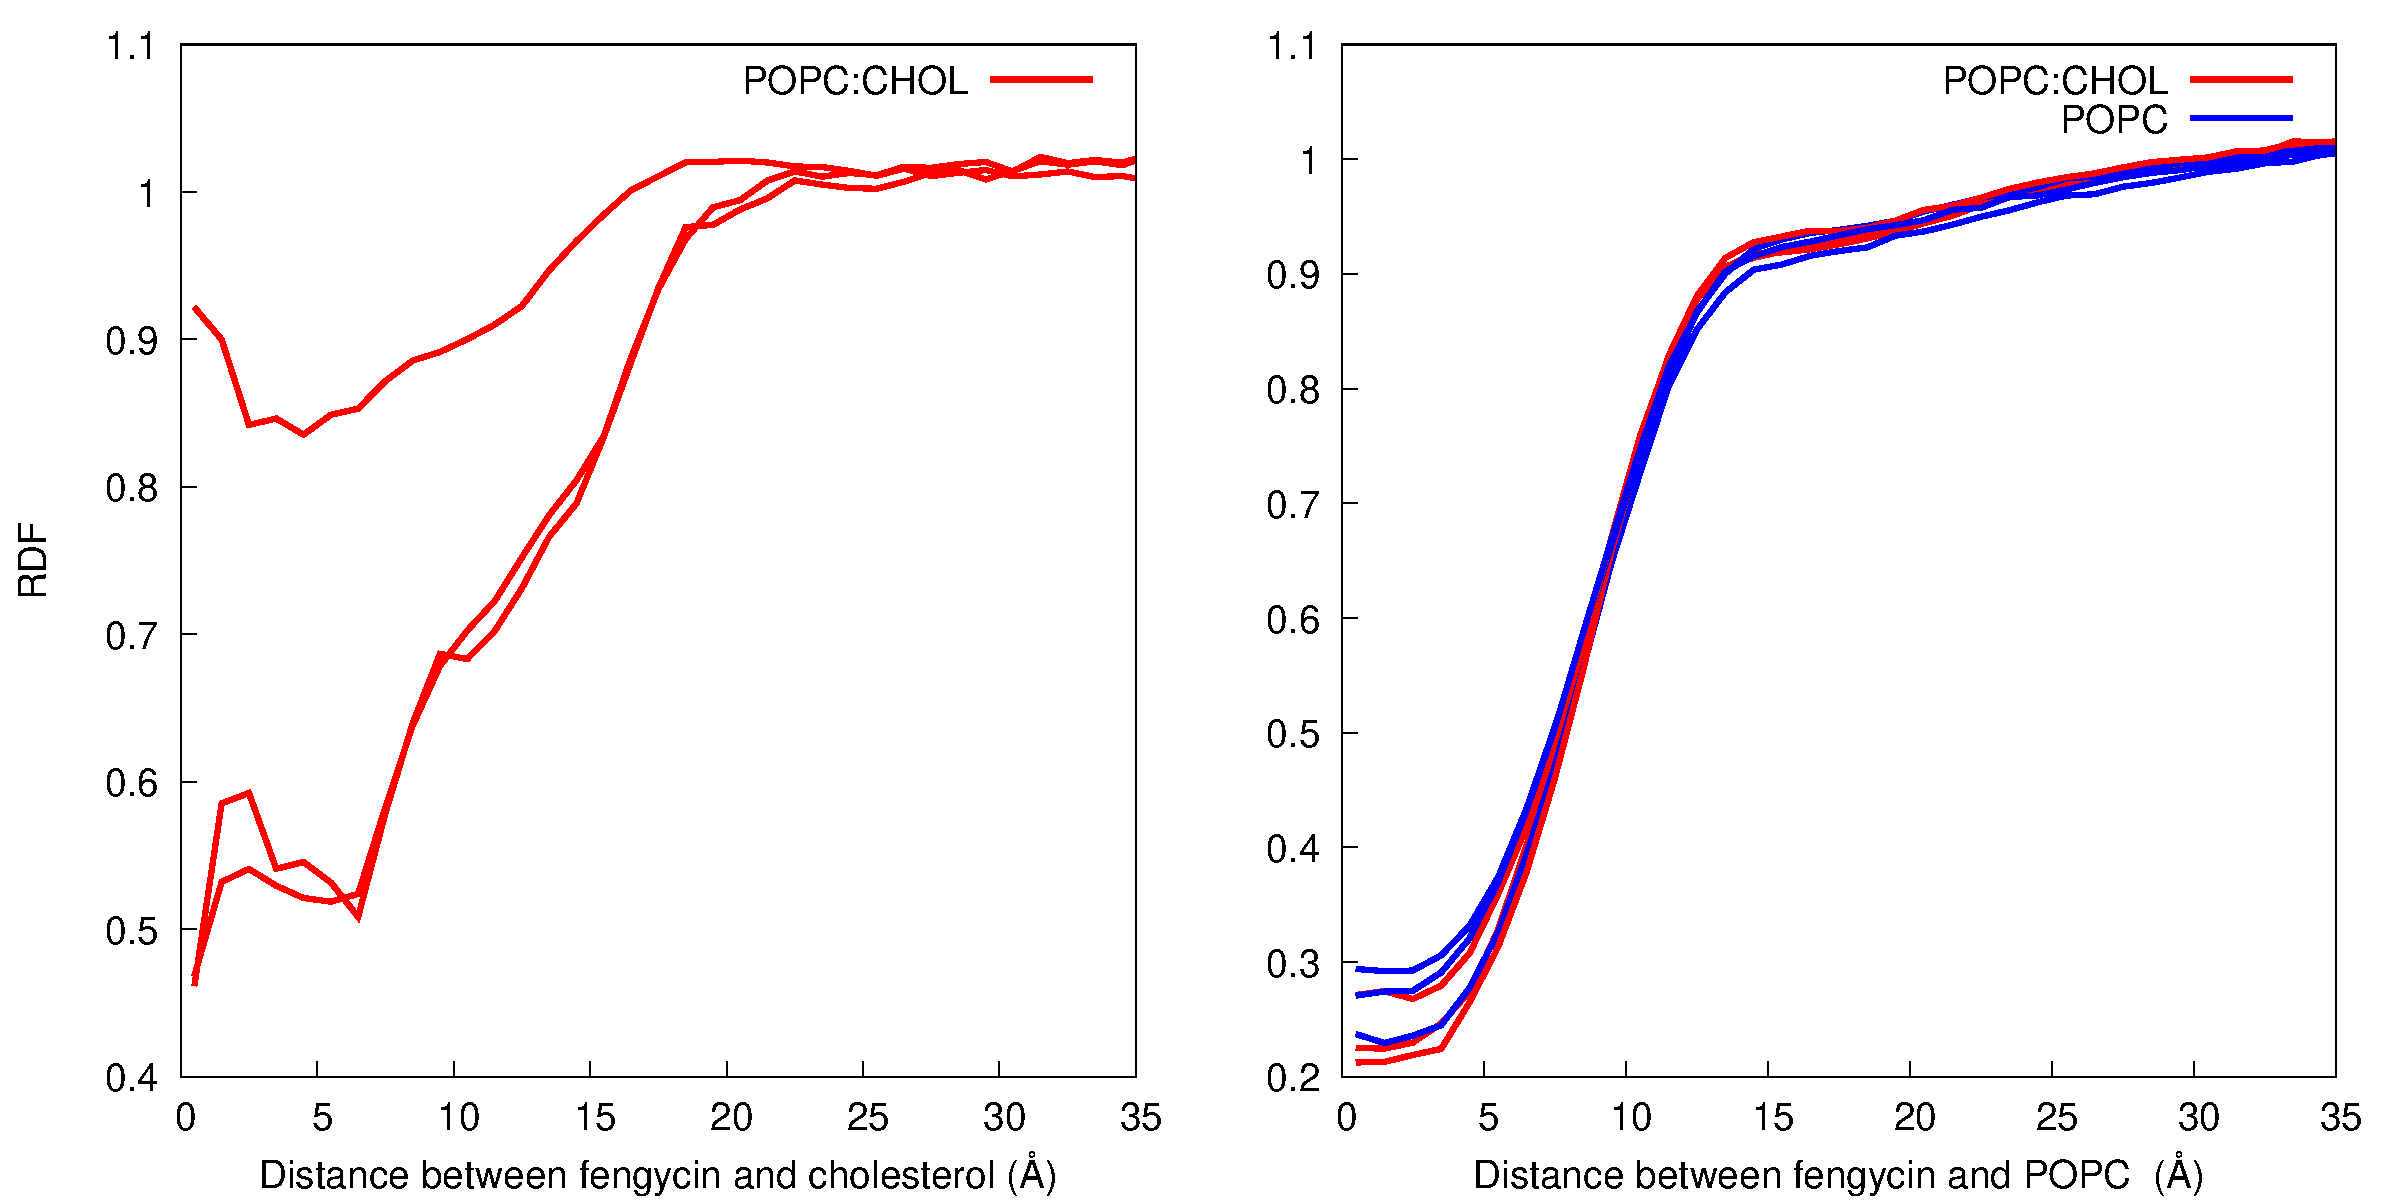
\includegraphics[width=1.0\textwidth]{chapter3_figs/xyrdf_all_fc_fp.pdf}
\caption{Lateral radial distribution function between A. cholesterol and fengycins. B. POPC and fengycins. Along y-axis is the radial distribution function and along the x-axis is the distance between fengycins and cholesterols/phospholipids. Same color curves refer to different replicates with similar system composition.}
\label{f:xyrdf_fc_fp}
\end{figure}

\subsection{Does cholesterol contribute to a better packing score?}
\label{ss:fl_packing}
Even though we do not observe any lipid/sterol preference around fengycins,
we wanted to know if lipids pack differently around fengycins depending on cholesterol's presence. In order to quantify lipid packing we used lipid/cholesterol-fengycin contacts 
using the methods \ref{sss:fl} as indicated in section \ref{s:methods}.
Fig \ref{f:ff_fl} suggests that increasing fengycin-fengycin contacts results in decreasing
fengycin-lipid contacts regardless of membrane composition. 
But in POPC:CHOL, the range of optimum contacts for both fengycin-fengycin (8-11) and 
fengycin-lipid(12-20) is broader compared to POPC. This suggests that in presence of cholesterol fengycins pack around themselves and around lipids more efficiently.
In absence of cholesterol there is some chance of higher fengycin-lipid 
contacts (22) which is suggestive of smaller aggregates in POPC bilayer being surrounded by lipids. Infact, this shows up in the difference 
%%%%Can we quantify the packing%%%%%
plot too where we see at low fengycin-lipid(8-10) contacts, higher fengycin 
aggregation observed in pure POPC. Additionally, higher fengycin-lipid contacts(20-22) prefer lower peptide aggregation in the absence of cholesterol which is not that probable in presence of cholesterol evident from figure \ref{f:ff_fl} difference plot. While an efficient optimum fengycin-fengycin and fengycin-lipid contacts are preferred in the presence of cholesterol as evident in the prominent blue color in the middle of difference plot suggesting better packing. This can lead to restricting the membrane disordering effects of fengycin to immediate surroundings of the lipopeptide in POPC:CHOL. 
\begin{figure}[h!]
\centering
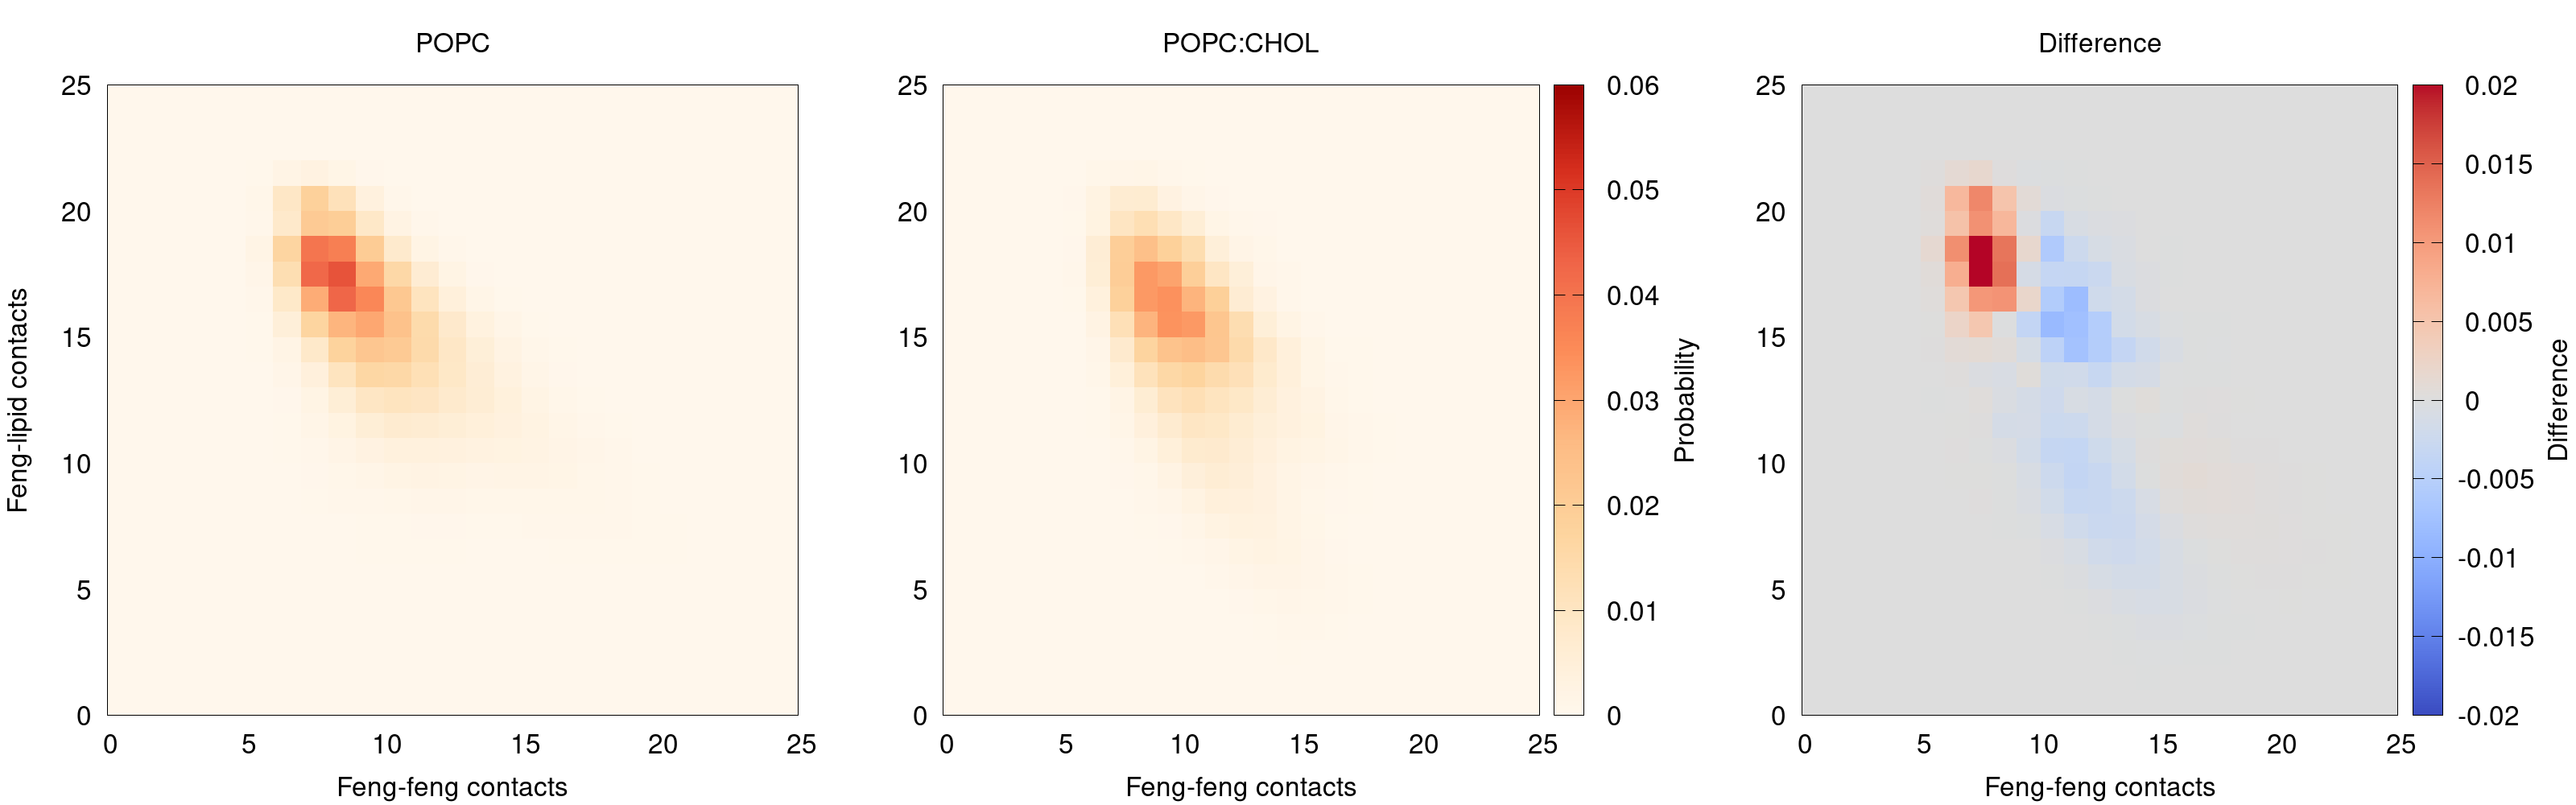
\includegraphics[width=6in,angle=0,keepaspectratio]{chapter3_figs/ff_fl_comb.png}
\caption{Probability of number of feng-feng contacts and number of feng-lipid contacts. 
A. POPC B. POPC-CHOL C. POPC-POPC:CHOL. We used the equations \ref{e:contact} and \ref{e:no_cont} to calculate the different contacts.}
\label{f:ff_fl}
\end{figure}

\subsection{No lipid/sterol demixing in POPC:CHOL}
Section \ref{ss:fl_packing} suggests efficient packing of lipids and sterols around 
fengycins. We are interested in any preference of lipids/sterols to be in higher concentration in presence of lipopeptides. The method \ref{sss:rdf} was used to plot figure \ref{f:xyrdf_cc_pc_pp}. The latter shows that there is no demixing between sterols and lipids and 
no tendencies to cluster between  sterols or lipids. This along with 
sections \ref{ss:fl_packing} and \ref{ss:no_fc_fp} suggests that the increase in 
lipid/sterol packing around fengycins in presence of cholesterol is non-specific to 
phospholipid or sterol and is a more of a general increase in packing. 
%%%%No lipid rafts%%%%%
This can attributed to the inherent ordering tendencies of 
cholesterol and a better packing of the overall membrane. 
%%%{Find a reference for this.}
This is consistent with the prediction that two or more phospholipids are required to observe demixing. %%%%\hl{Find reference.}

\begin{figure}[h!]
\centering
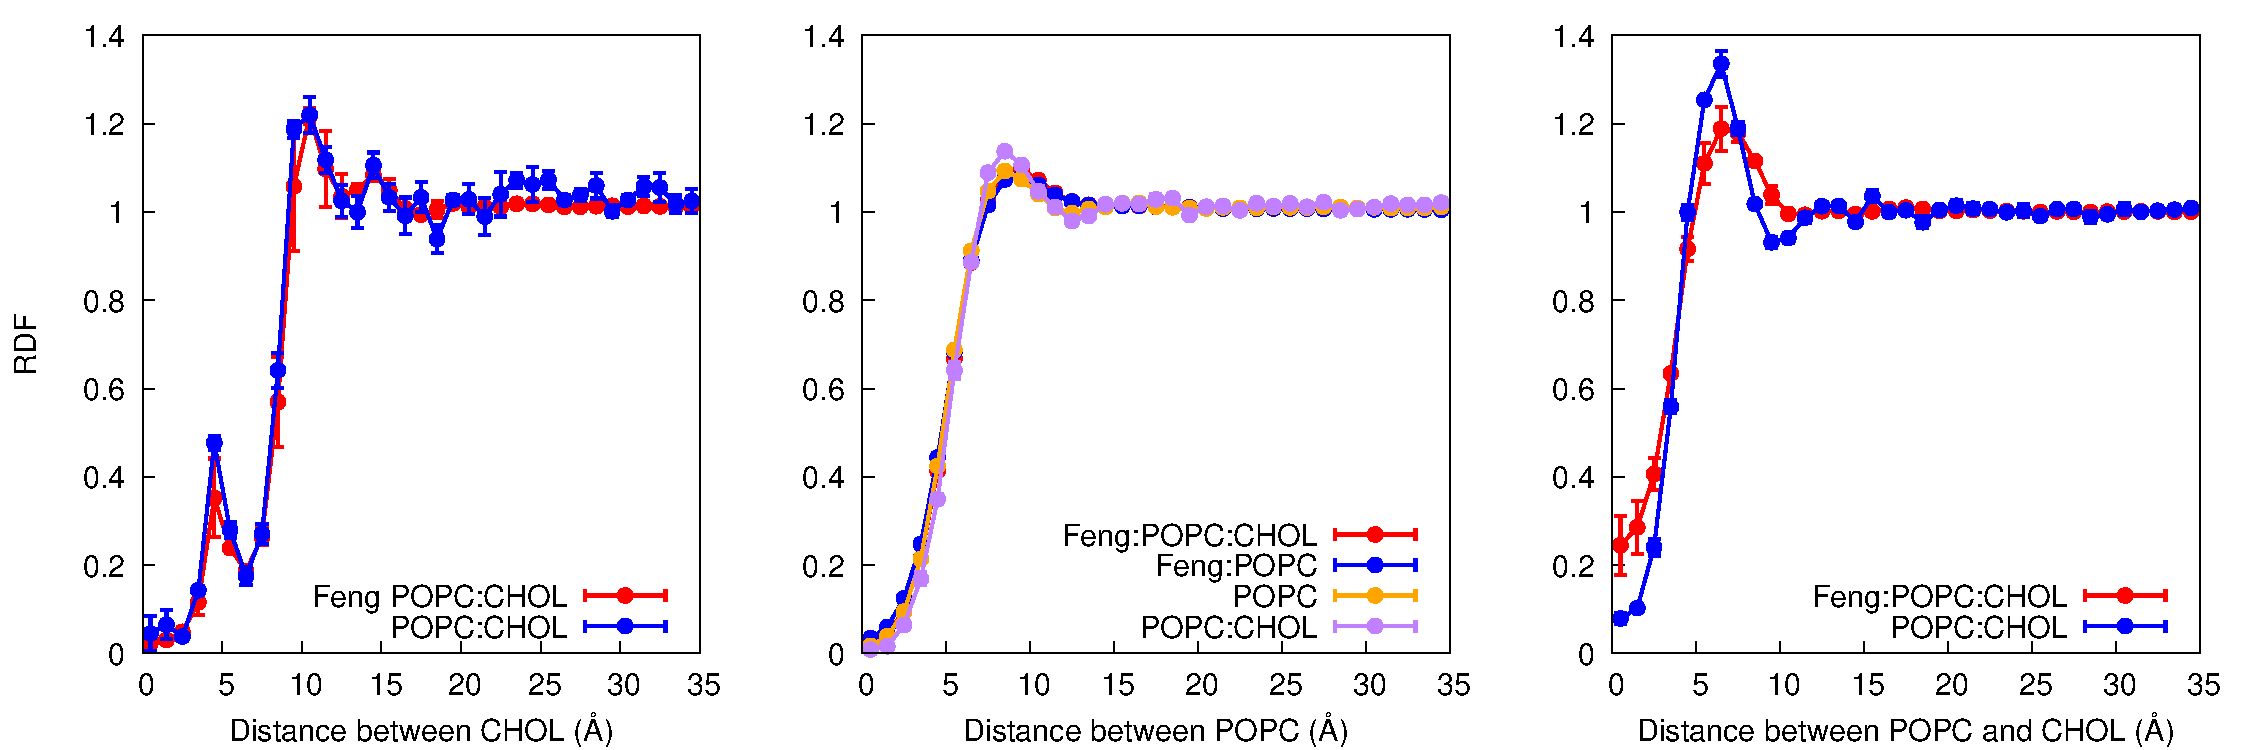
\includegraphics[width=6in,angle=0,keepaspectratio]{chapter3_figs/xyrdf_all_cc_pc_pp.pdf}
\caption{Lateral radial distribution function between A. cholesterols B. POPCs C. POPC and Cholesterol 
All the lipid-lipid radial distribution functions are compared to their analogous value with no fengycins present. The cholesterol's radial distribution function is noisy when fengycin is absent since we have of only 800nanosecond of data.}
\label{f:xyrdf_cc_pc_pp}
\end{figure}

\subsection{Cholesterol orders the membrane}
Cholesterol in membrane makes the membrane more ordered but yet flexible \cite{Barenholz2002}.
In Figure \ref{f:dibmop_1d}A we looked at the molecular order parameters for the 
phospholipid chains with respect to distance from fengycins. We used the method in 
section \ref{sss:mol_ord} to calculate the molecular order parameters.
Figure \ref{f:dibmop_1d}A suggests that the trend for order parameters are similar in 
the presence/absence of cholesterol. There is a dip in order parameter next to 
fengycins but as we move away from the lipopeptides there is a higher ordering effect 
when cholesterol is present. In addition at long range we find the molecular order 
parameters are much higher in presence of cholesterol. Figure \ref{f:dibmop_1d}B is 
computed by subtracting the system with no fengycins from the system with 
lipopeptides data. Since the y-axis for the \ref{f:dibmop_1d}B is negative all along for 
figure \ref{f:dibmop_1d}B implying that absolute difference is smaller for phospholipid 
order parameters in the presence of cholesterol and fengycins compared 
to no fengycins. Hence even though fengycins are present the disordering effects on phospholipids are much lower when cholesterol is present. This can be attributed 
to the inherent properties of cholesterol trying to force the phospholipid tails 
to be parallel to the membrane normal.
\begin{figure}[h!]
\centering
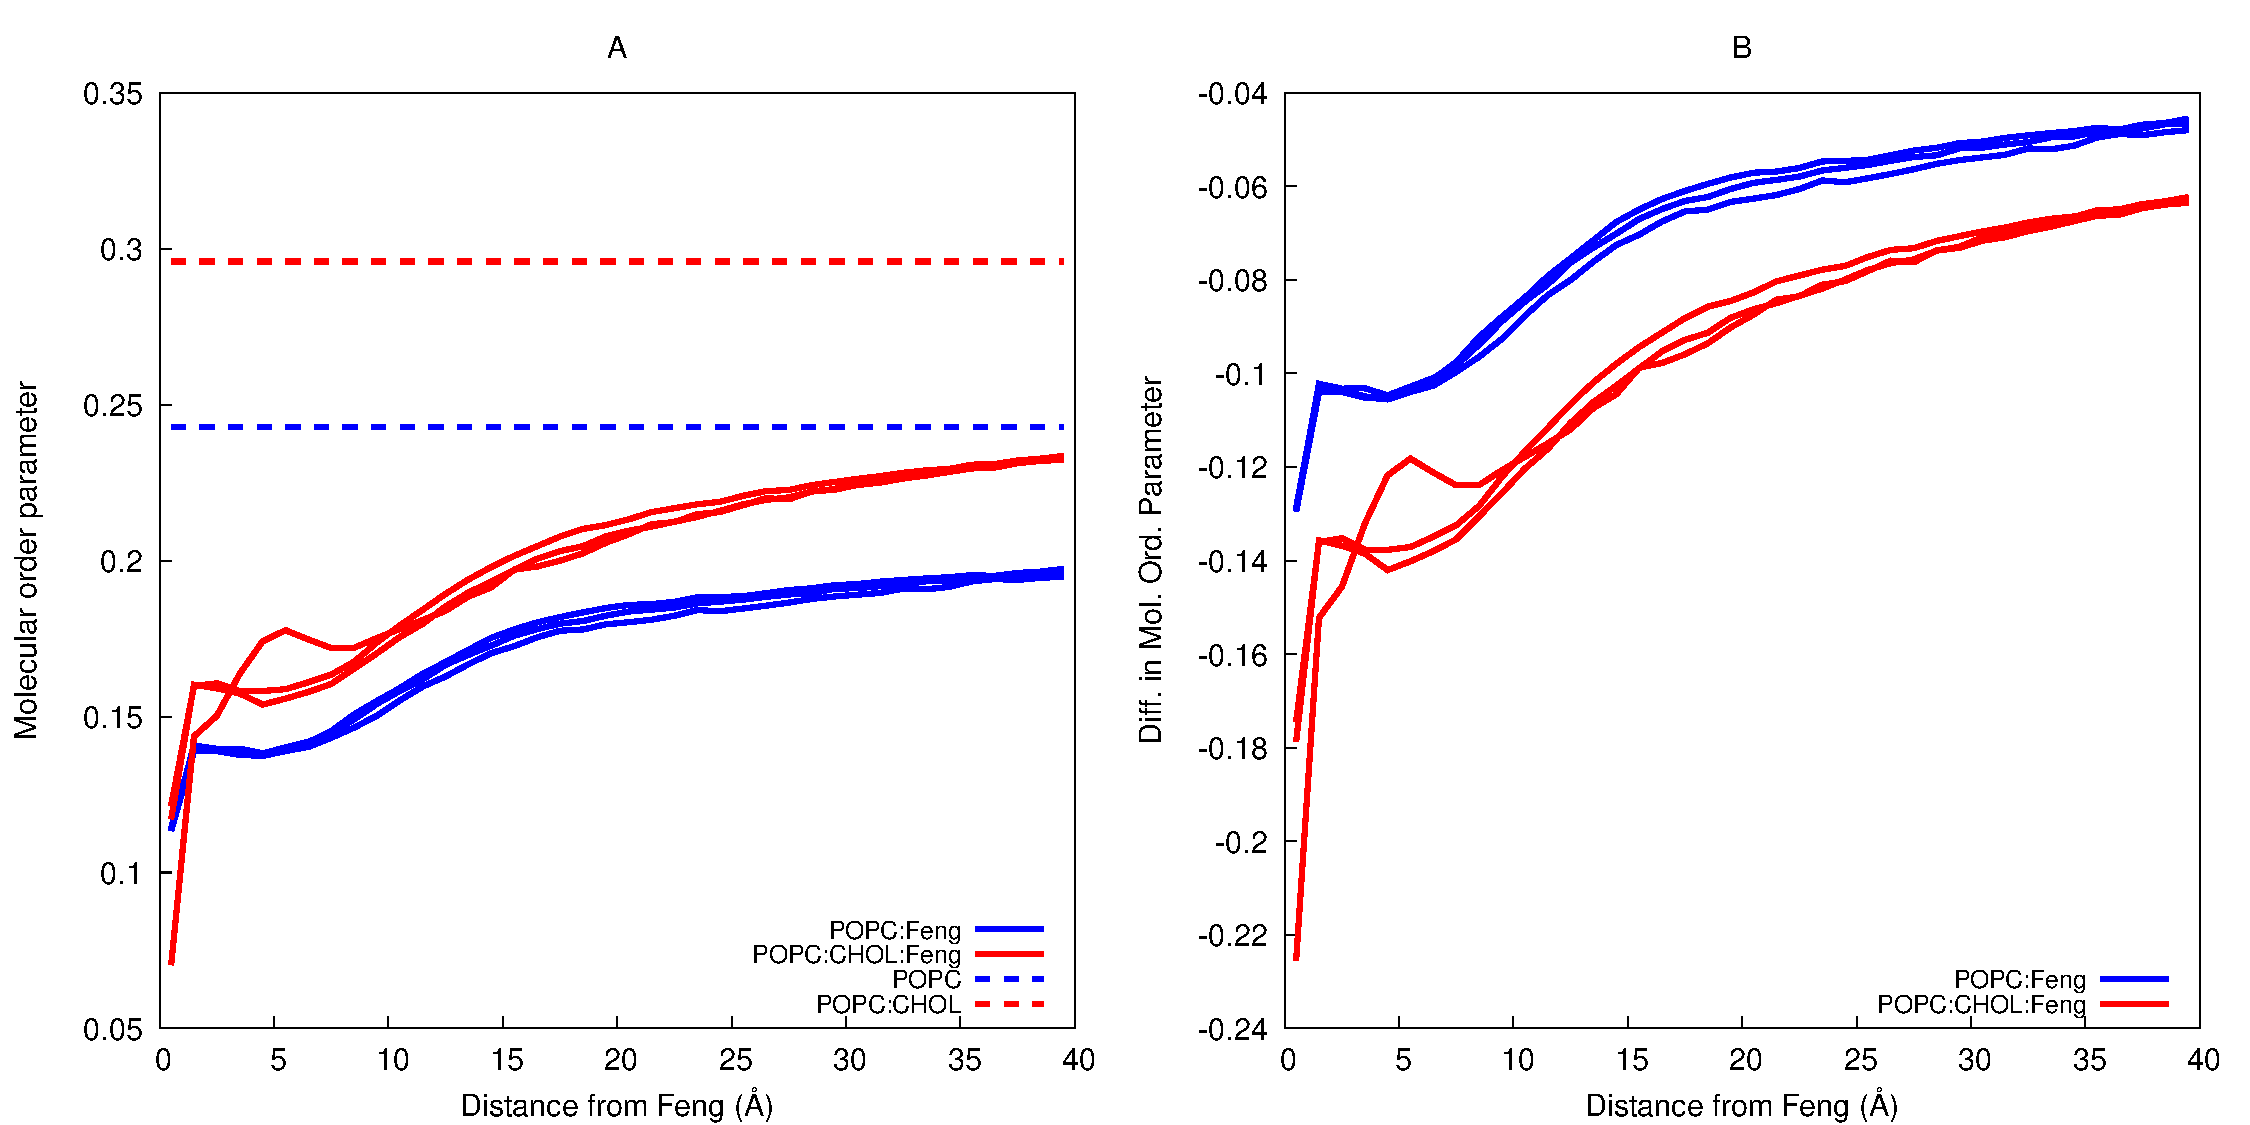
\includegraphics[width=4.5in,angle=0,keepaspectratio]{chapter3_figs/dibmop_avg_1d.pdf}
\caption{Molecular order parameters. A. Weighted average molecular order parameters as a function of distance from fengycins. B. Fengycins - no fengycins. Each curve shows the weighted average in each 
replicate. }
\label{f:dibmop_1d}
\end{figure}
%%%%%%%Woohoo order parameters are high%%%%%%%%
Next, we also looked at how the molecular order parameters change with aggregation 
of fengycins. In figure \ref{f:dibmop_2d} we see molecular order parameter with 
respect to fengycin-fengycin contacts. The general trend is higher the 
fengycin-fengycin contacts meaning higher aggregation results in reduced molecular 
order parameters for lipids next to fengycins.
However we observe that in presence of cholesterol the order parameters are higher compared to pure POPC at a similar distance from the fengycins. And in the absence of fengycins the lowered order parameters extend to a longer distance from fengycins.
This suggests that the disordering effects of fengycins increase with aggregation to much longer range in absence of cholesterol. For instance, the value of order parameter is low even at 20-25 \AA from fengycin at the highest fraction of fengycin-fengycin contacts in pure POPC compared to POPC:CHOL where a similar molecular order parameter value observed at 10 \AA distance from fengycins. In essence the damage control improves in cholesterol rich membranes and thus inhibits fengycin from leaking the membrane.
\begin{figure}[h!]
\centering
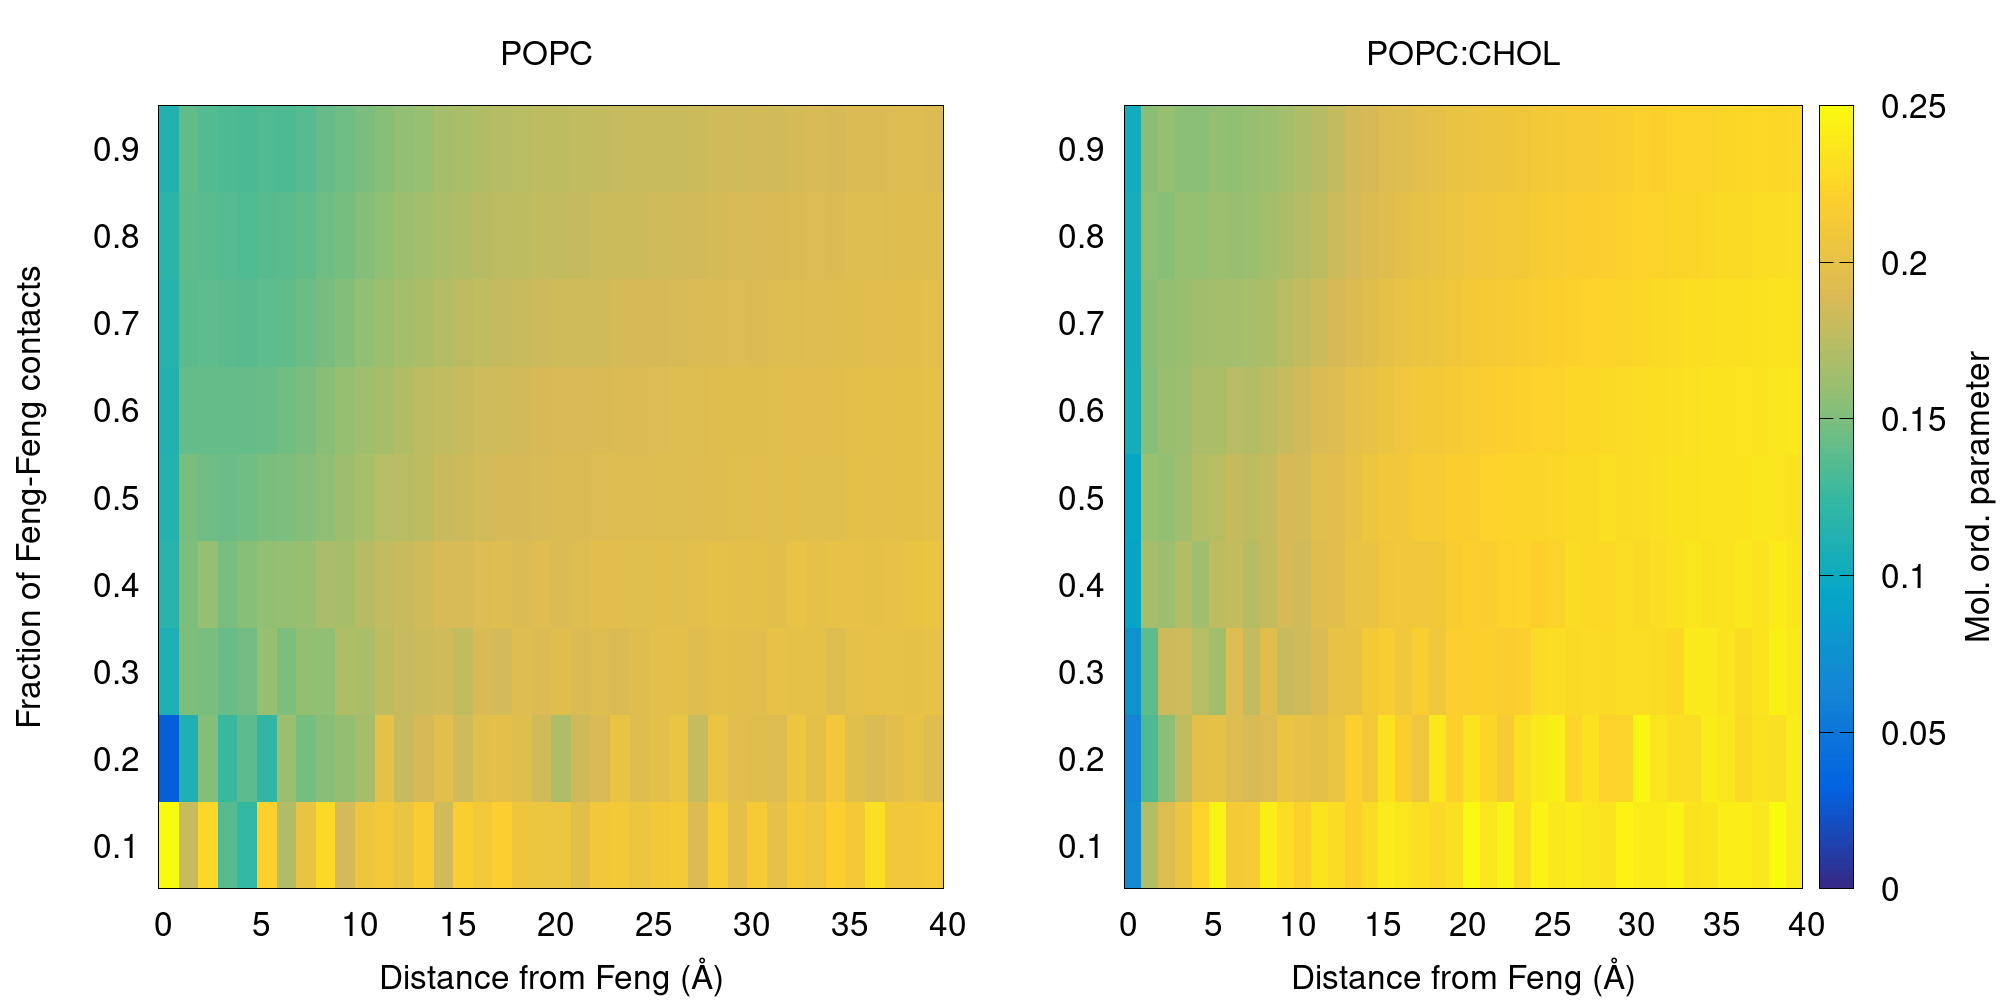
\includegraphics[width=6in,angle=0,keepaspectratio]{chapter3_figs/dibmop_avg_2d.png}
\caption{Weighted average molecular order parameters as a function of distance from fengycins and fraction of fengycin-fengycin contacts.(A) POPC (B)POPC:CHOL. Along x-axis is the distance from fengycins, y-axis is the fraction of fengycin-fengycin contacts and the color range indicates the molecular order parameters. }
\label{f:dibmop_2d}
\end{figure}
\subsection{Fengycin bends the membrane}
According to Horn et al more the bending of the membrane 
higher is the probability that membrane will leak \cite{Grossfield2013}
If fengycins disorders the lipids we wanted to know how the presence of cholesterol 
affects bending of the membrane. Qualitatively, when we looked at the different 
frames of the trajectory we could see that the membrane was bending around a large 
fengycin aggregate. In order to quantify that we calculated the height of 
phospholipid heads with respect to distance from fengycins using the method outlined
in section \ref{sss:z-dist}.
%%%%Bending in membrane due to lipopeptides%%%%%%%%%
Following that we subtracted the total average height of the phospholipid heads from 
the lipopeptide distance dependent histogram of phospholipid heads and obtained the figure 
\ref{f:z-hist} featuring both membrane leaflets.
In order to refresh your memory, all my systems had fengycins bound to only upper leaflet. 
 Positive z-height for phospholipid suggest that the lipid  are higher than the 
 average phosphate heights for that membrane leaflet. Since, the phospholipid height is 
 positive for systems with cholesterol right next to the fengycins or right under it, this 
 means that the membrane has a convex curvature for those systems. On the other hand for 
 pure POPC, the height of phospholipids is not that high in the upper leaflet but it is 
 much higher in the lower leaflet. This suggests both slight convex bending and thinning of
 the  membrane around fengycins in POPC.
 We know that cholesterol is observed to be present in regions with more membrane bending 
 and this suggests that the bending in cholesterol rich systems is normal. But due to 
 membrane thinning in absence of cholesterol indicates membrane-leakage can be more
 prone in absence of cholesterol.
\begin{figure}[h!]
\centering
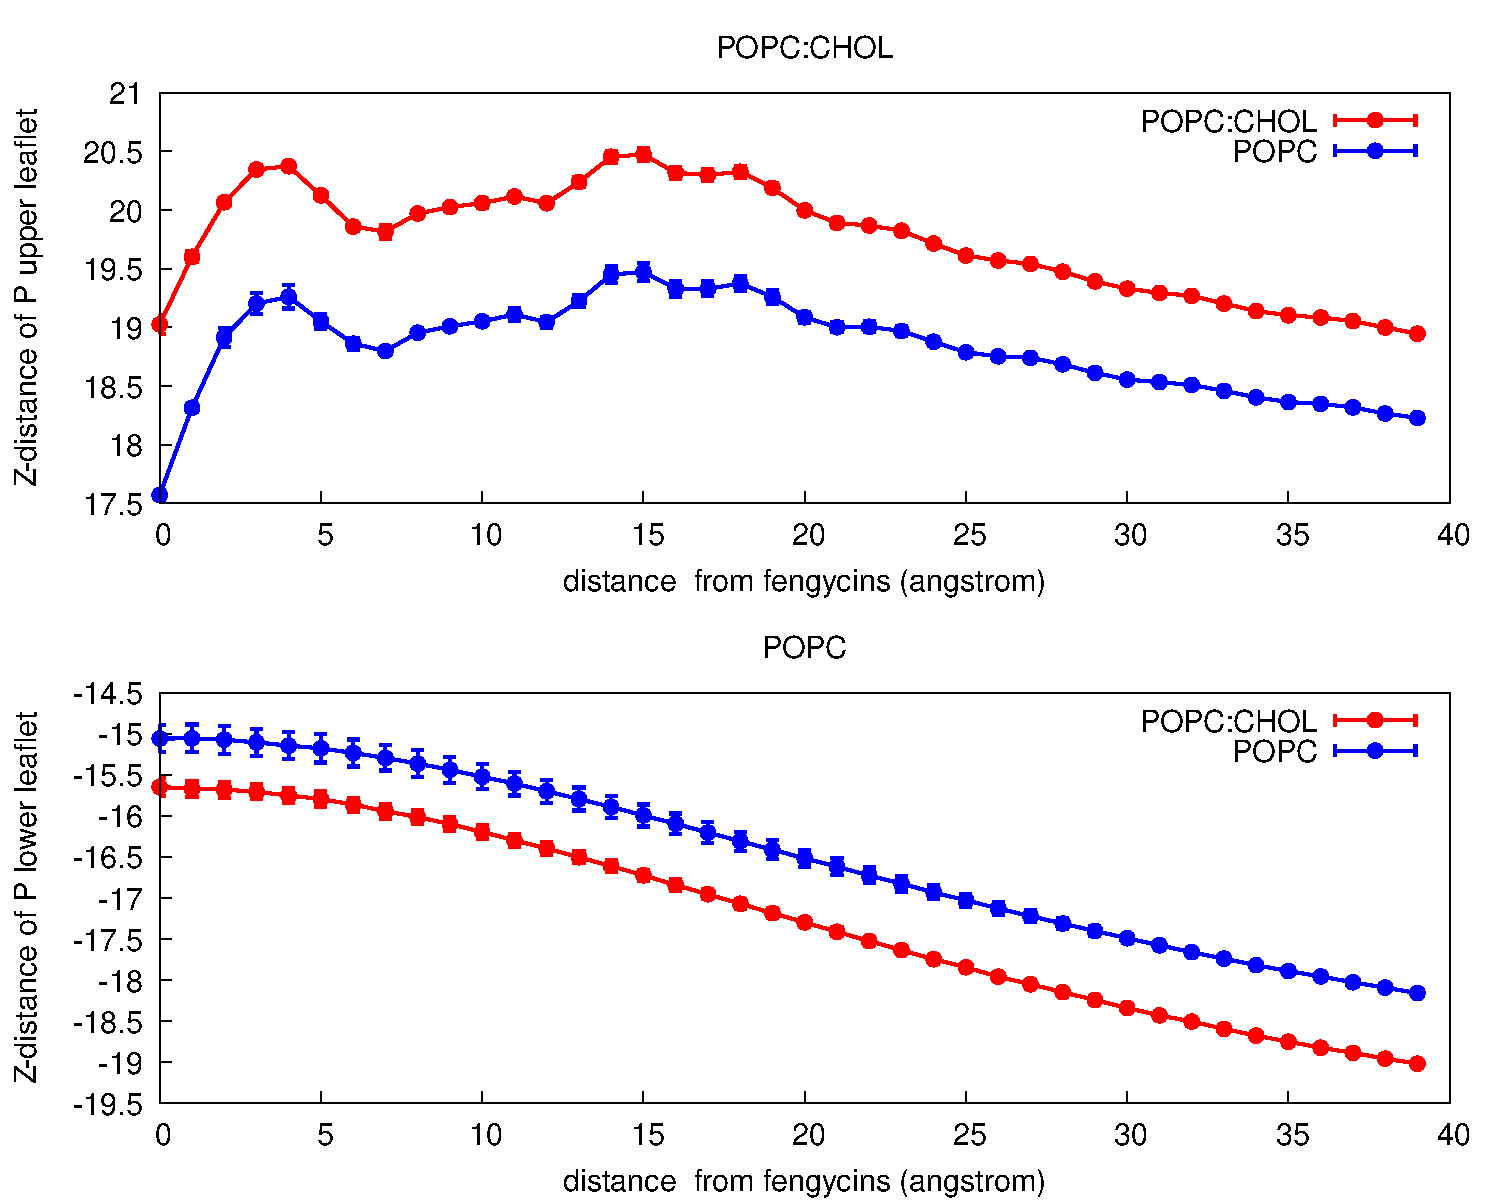
\includegraphics[width=5.0in,angle=0,keepaspectratio]{chapter3_figs/z-hist.pdf}
\caption{A. Z-distance of upper bilayer phosphates as a function of distance from fengycins. B. Z-distance of lower bilayer phosphates as a function of distance from fengycins. 
Along x-axis is the distance of phospholipid from fengycin. Y-axis denotes the height of phospholipids after taking into account the thickness of the membrane. The top plot is for the upper leaflet and the bottom one is for the lower leaflet. Each weighted ensemble run is considered as a single measurement and standard error is calculated using this assumption. }
\label{f:z-hist}
\end{figure}

\section{Discussion}

Our results suggest that the specificity of fengycins in 
presence or absence of cholesterol is dependent on the aggregation of fengycin.
But the differences in aggregation is subtle. In presence of cholesterol
larger aggregates with better packing preferred.
In pure POPC a variety of aggregate sizes are observed and not just bigger aggregates.
The lipid packing around fengycins increases in presence of cholesterol
but there is no specific preference for either phospholipid or cholesterol.
We also found that cholesterol orders the membrane even in presence of lipopeptides. 
On the other hand in pure POPC, the disordering effects of fengycin are more pronounced to a
longer range with increase in aggregation.
While in cholesterol's presence the disordering effects are more contained. This can be 
attributed to better packing of lipids and the inherent tendency of cholesterol to order the
membrane. But cholesterol induces a more concave bending of the membrane while its absence 
causes more of a membrane thinning. Thus our results show that the effects of cholesterol on
fengycin inhibition is due to more of the inherent properties of cholesterol that makes the 
membrane more flexible yet ordering the lipids. 
And this can be additionally seen even with ergosterols which have very similar structures 
to cholesterol.
In fact Mantil et al also found that ergosterol may be buffering the membrane disordering 
effects of fengycin \cite{MantilAvis2019,MantilTyler2019}.
Also, presence of ergosterol in fungal membranes reduces the efficacy of fengycin which 
shows its ineffectiveness against certain fungal species
%%%%\hl{Find the references from Mantil 
%%%%papers}

Thus we can say that the reason there is less membrane leakage for Fiedler et al 
\cite{Heerklotz2015} was because 
cholesterol creates an ordered lipid phase where even after binding the membrane disordering
due to fengycins is short range and thus the membrane can have more and more fengycin uptake
without causing the equivalent damage with absence of cholesterol.
In fact the high aggregation propensity may be also a packing issue. Due to the presence of
cholesterol, like POPC the tails are forced to be parallel to the membrane. This means
smaller distance between fengycins and thus the number of contacts are higher and due to
dense packing there is more propensity to aggregate and remain in that state.

Overestimation of protein-protein dimerization free energy seen for water soluble proteins 
using MARTINI model results in peptide precipitation in water below the solubility limit 
\cite{Elcock2013}. This is true even after reparametrizing the protein 
force-field\cite{Marrink2013}. In fact it was found that the protein-protein dimerization 
for improved protein forcefield was not validated against experimental data 
\cite{Nishizawa2014}.
Thus, in spite of some statistically significant differences in aggregation of fengycins in 
the presence/absence of cholesterol, the inherent tendency of MARTINI forcefield to 
overestimate dimerization, lead us to believe that all-atom simulations of a similar system 
would be needed to better characterize the aggregate structure.
Also the new ergosterol MARTINI parameters were derived from cholesterol parameters 
\cite{Melo2015}. Thus to compare two different sterols we need weighted all-atom models 
to capture the implications on the membrane due to their structural differences.

Going forward, we would like to perform the weighted ensemble simulations of fengycin micelles binding to the membrane. This would help us determine if the membrane ordering effects of cholesterol changes the binding free energy of fengycins.

\section{Conclusions}
\label{s:conc}
Our simulations provide a more detailed picture of implications of fengycin aggregation 
on the lipid membrane. It corroborates with the broader result suggested by Fiedler et al \-- that fengycins cause less leakage in cholesterol rich systems. But the individual lipid-protein interactions hypothesized by them were not observed in our simulations. 
But we observed more subtle changes in lipid packing around fengycins, more ordering of the membrane and containing the membrane disordering effects by cholesterol.
This suggested that the membrane leakage in pure POPC due to fengycins is due to the absence of buffering by cholesterol in terms of membrane ordering.

